La solución implementada en el laboratorio para el sistema del coche autónomo se basa en la utilización de diferentes tecnologías de conectividad. En primer lugar, la red 4G se emplea como el medio principal de conexión entre todos los elementos del sistema. El coche autónomo está equipado con un módem y una tarjeta SIM, lo que le proporciona conectividad a la red 4G.
En cuanto al móvil, se plantean dos opciones de conexión para que el usuario pueda comunicarse con el coche. La primera opción consiste en utilizar una tarjeta SIM en el móvil, lo que permite aprovechar la conectividad 4G para establecer comunicación con los demás componentes del sistema. La segunda opción es conectar el móvil a la red del laboratorio a través de Wi-Fi. Si hay una red Wi-Fi disponible, el móvil puede conectarse a ella y tener acceso a internet. Esto ofrece la posibilidad de utilizar servicios en línea y comunicarse mediante aplicaciones conectadas a internet. La calidad de la conexión dependerá de la red Wi-Fi disponible en el entorno.
Además, se utiliza un cliente Mosquitto en el móvil, lo cual permite establecer una comunicación bidireccional entre el coche y el servidor ubicado en el ordenador. Mosquitto es un software de mensajería MQTT (Message Queuing Telemetry Transport) ampliamente utilizado en la comunicación entre dispositivos IoT (Internet de las cosas). Esta comunicación bidireccional permite el intercambio de datos y comandos entre el coche y el servidor.
Por último, el ordenador que aloja la inteligencia artificial (IA) se conecta a la red del laboratorio, lo cual garantiza una mayor estabilidad y ancho de banda. Esta conexión es fundamental para el procesamiento de datos intensivo requerido por la IA. Al estar conectado a la red del laboratorio, el ordenador puede acceder a recursos compartidos, bases de datos y servicios en la nube necesarios para el funcionamiento y entrenamiento de los modelos de inteligencia artificial.
En resumen, la solución implementada utiliza la red 4G para la conexión entre los elementos del sistema. El móvil puede conectarse al coche autónomo mediante una tarjeta SIM o mediante Wi-Fi del laboratorio. El cliente Mosquitto en el móvil facilita la comunicación bidireccional con el servidor en el ordenador. Por su parte, el ordenador se conecta a la red del laboratorio para aprovechar la estabilidad y el ancho de banda necesarios para el procesamiento de datos de la IA.

\begin{figure}[H]
\centering
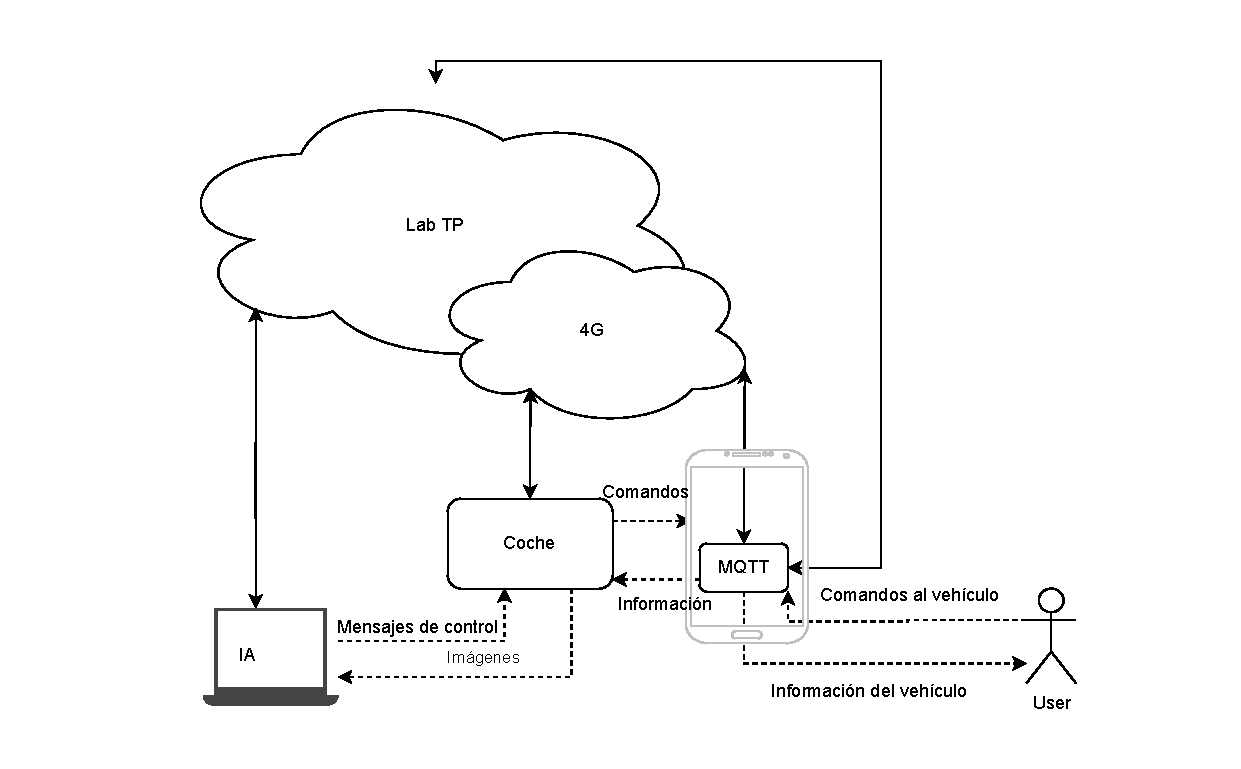
\includegraphics[width = \textwidth]{Imagenes/Solucion/12.pdf}
\caption{Infraestructura del sistema en el laboratorio}
\label{12}
\end{figure}

En cuanto a la red 4G, según el estándar, estará formada por un eNodeB (estación base) y un core de red. En nuestra configuración, ambos elementos se ejecutarán en el mismo ordenador (en el que también se encuentra el servidor mosquitto) El eNodeB será responsable de la comunicación inalámbrica con los dispositivos móviles, mientras que el core de red gestionará el enrutamiento y la conexión con otros sistemas.
En nuestra implementación, utilizaremos la interfaz de red de Blade como interfaz radio para el eNodeB. La Blade actuará como la interfaz de red entre la red 4G y los otros componentes del sistema, permitiendo la comunicación bidireccional.
La interfaz SGi (interfaz de servicio de paquetes entre el core de red y la red externa) nos brinda acceso a los recursos y servicios de Internet, lo que permitirá tener conexión entre la red 4G e Internet.
En resumen, en nuestra solución, el ordenador actuará como un eNodeB y core de red 4G, ejecutando ambos componentes en el mismo sistema. Blade será la interfaz de red utilizada para la comunicación con el eNodeB, mientras que la conexión a Internet se establecerá a través de la red SGi. Esta configuración nos permitirá gestionar y controlar la red 4G y acceder a servicios externos a través de la conexión a Internet.

\begin{figure}[H]
\centering
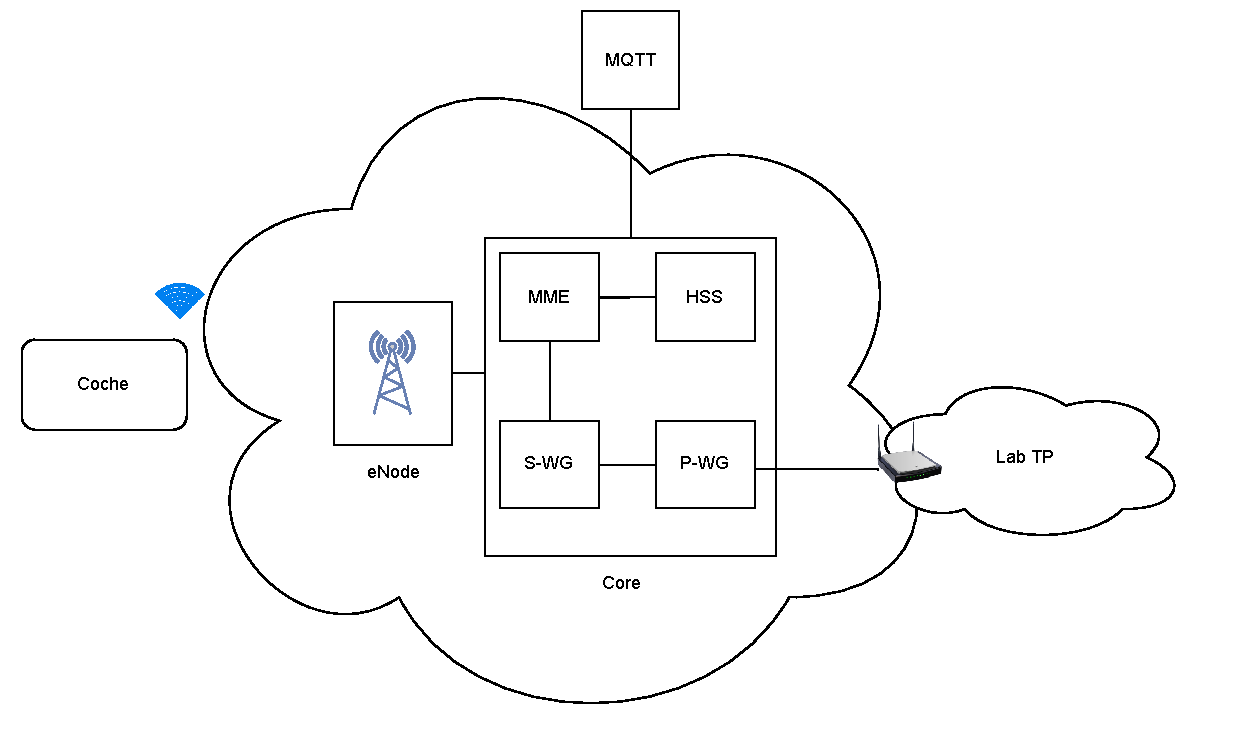
\includegraphics[width = \textwidth]{Imagenes/Solucion/11.pdf}
\caption{Infraestructura de la red 4G en el laboratorio}
\label{11}
\end{figure}

